\section{Spécifications Techniques}


\subsection{Évaluation comparative des technologies.}
\begin{frame}{Choix pour API Gateway}
    \begin{figure}[H]
        \centering
        \begin{minipage}{0.32\textwidth}
            \centering
            
\includegraphics[height=3cm]{assets/images/spring.png}
        \end{minipage}%
        \hspace{0.03\textwidth}
        \begin{minipage}{0.32\textwidth}
            \centering
            
\includegraphics[height=3cm]{assets/images/laravel.png}
        \end{minipage}%
        \hspace{0.03\textwidth}
        \begin{minipage}{0.32\textwidth}
            \centering
            
\includegraphics[height=3cm]{assets/images/django.png}
        \end{minipage}
    \end{figure}
\end{frame}

\begin{frame}{Benchmark Fronted}
    \begin{figure}[H]
        \centering
        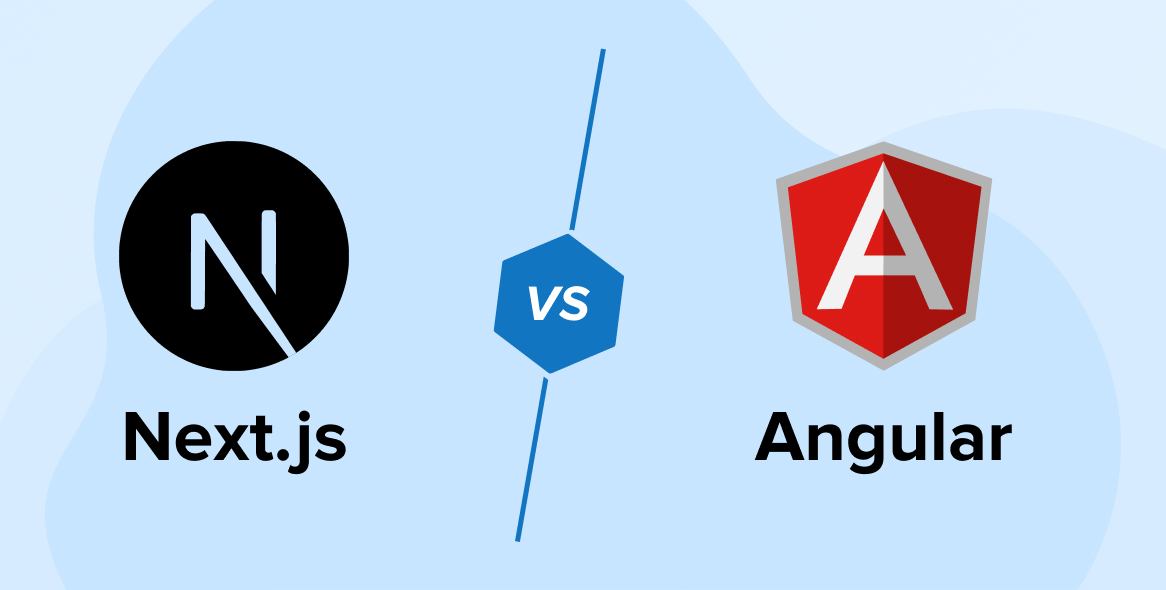
\includegraphics[height=5cm]{assets/images/bench-next.jpg}
    \end{figure}
\end{frame}

\begin{frame}{Benchmark model IA}
    \begin{figure}[H]
        \centering
        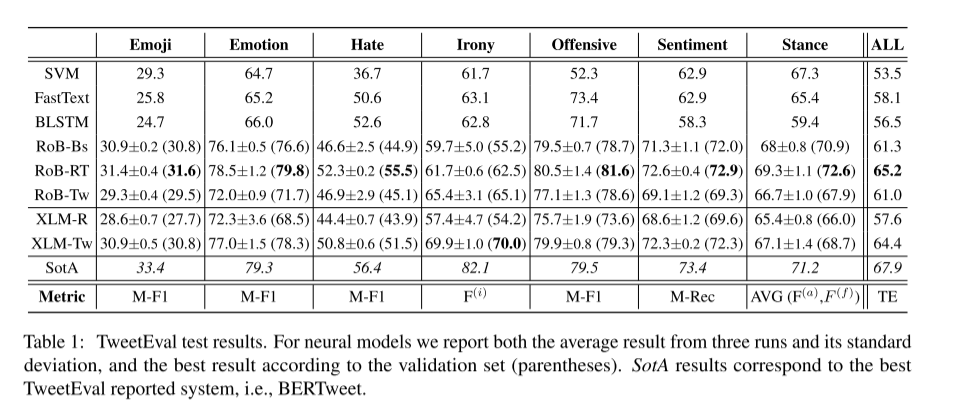
\includegraphics[height=6cm]{assets/images/ai-acc-dataset.png}
    \end{figure}
\end{frame}

\subsection{Technologies Sélectionnées}
\begin{frame}{Technologies choisies pour les services}
    \begin{figure}[H]
        \centering
        \begin{minipage}{0.32\textwidth}
            \centering
            
\includegraphics[height=3cm]{assets/images/next.png}
        \end{minipage}%
        \hspace{0.03\textwidth}
        \begin{minipage}{0.32\textwidth}
            \centering
            
\includegraphics[height=3cm]{assets/images/spring.png}
        \end{minipage}%
        \hspace{0.03\textwidth}
        \begin{minipage}{0.32\textwidth}
            \centering
            
\includegraphics[height=3cm]{assets/images/keycloak.png}
        \end{minipage}

    \end{figure}
\end{frame}



\begin{frame}{Technologies choisies pour IA}
    \begin{figure}[H]
        \centering

        \begin{minipage}{0.5\textwidth}
            \centering
            
\includegraphics[height=2cm]{assets/images/tinyllama.png}
        \end{minipage}
        \hspace{0.1\textwidth}
        \begin{minipage}{0.5\textwidth}
            \centering
            
\includegraphics[height=2cm]{assets/images/langchain.jpeg}
        \end{minipage}
        \hspace{0.1\textwidth}
        \begin{minipage}{0.5\textwidth}
            \centering
            
\includegraphics[height=2cm]{assets/images/mongo.png}
        \end{minipage}
    \end{figure}
\end{frame}

\subsection{Communication entre services}
\begin{frame}{Communication entre services}
    \begin{figure}[H]
        \centering
        
\includegraphics[height=2cm]{assets/images/rest.png}
        \hspace{0.1\textwidth}
        
\includegraphics[height=2cm]{assets/images/kafka.png}
    \end{figure}
\end{frame}

\subsection{Conclusion}
\begin{frame}{Conclusion}

    En bref, notre application de classification de sentiments des commentaires Hespress utilise une architecture microservices avec Next.js (front), FastAPI (back), Spring (API Gateway), Keycloak (auth), PostgreSQL, Redis (cache), Selenium (scraping) et le modèle cardiffnlp/twitter-xlm-roberta-base-sentiment. Ce projet a été réalisé durant mon stage au centre de formation Code 212.
\end{frame}
